\documentclass{standalone}
\usepackage{amsmath,amssymb,amsthm}
%%\usepackage[usenames,dvipsnames,table]{xcolor}
%%\usepackage{graphicx} 										% Graphics
\usepackage{tikz} \usetikzlibrary{calc,arrows.meta,intersections,patterns} 	% Figure
\usepackage{pgfplots}

%% !TEX root = ThesisManuscript_SJ.tex
%%
%%
%%	COLORS
%%_______________________________________________
\definecolor{MyBlue}{RGB}{0,120,155}
\definecolor{MyDarkBlue}{rgb}{0, 0.25, 0.45}
\definecolor{MyBrown}{rgb}{0.28, 0.20, 0.20}
\definecolor{MyOrange}{RGB}{255,80,30}
\definecolor{MyOldOrange}{rgb}{0.75, 0.25, 0.0}
\definecolor{MyRed}{RGB}{200,0,0}
\definecolor{MyGray}{RGB}{200,200,200}
\definecolor{MyGreen}{rgb}{0.33, 0.5, 0.18}
\definecolor{MyDarkGreen}{rgb}{0.15, 0.25, 0.18}
\definecolor{MyTurquoise}{rgb}{0, 0.4, 0.4}
\definecolor{MyViolet}{rgb}{0.44, 0.16, 0.39}
\definecolor{MyYellow}{rgb}{1, 0.65, 0}

\begin{document}
\centering

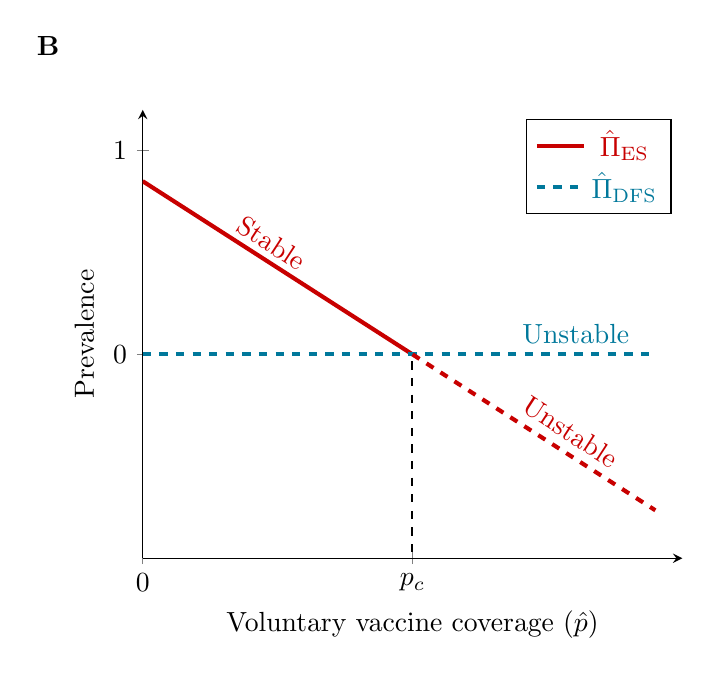
\begin{tikzpicture}
\begin{axis}[
    axis lines = left,
    xlabel = {Voluntary vaccine coverage ($\hat{p}$)},
    ylabel = {Prevalence},
    xtick={0,1},
    xticklabels = {0,$p_c$},
    ytick={0,1},
    xmax=2,
    ymin=-1.0,
    ymax=1.2,
    line width = {0.5pt},
%    xmajorgrids=true,
%    ymajorgrids=true,
%    legend pos=outer north east
]
%% Stable ES
\addplot [
    domain=0:1, 
    samples=2, 
    line width = 1.5pt,
    color = MyRed,
    ]
    {- 0.85*x + 0.85};
\addlegendentry{\textcolor{MyRed}{$\hat{\Pi}_{\rm ES}$}}
%% Unstable DFS
\addplot [
    domain=0:1.9, 
    samples=2, 
    color = MyBlue,
    line width = 1.5pt,
    style = dashed,
]
{0};
\addlegendentry{\textcolor{MyBlue}{$\hat{\Pi}_{\rm DFS}$}}
%% Unstable ES
\addplot [
    domain=1:1.9, 
    samples=2, 
    line width = 1.5pt,
    color = MyRed,
    style = dashed,
    ]
    {-0.85*x + 0.85};
%\addlegendentry{\textcolor{MyRed}{$\Pi_{\rm ES}$}}

%
\end{axis}
	\draw (-1.2,6.5) node (B) {\bf B};
	\draw (3.42,2.5) [dashed,line width=0.5pt] -- (3.42,0);
        	\draw (5.5,2.6) node (UDFS)[above, color=MyBlue] {Unstable};
	\draw (5.3,1.4) node (UES)[above, rotate=-33, color=MyRed] {Unstable};
	\draw (1.5,3.8) node (SES)[above, rotate=-33, color=MyRed] {Stable};
\end{tikzpicture}

\end{document}
%
